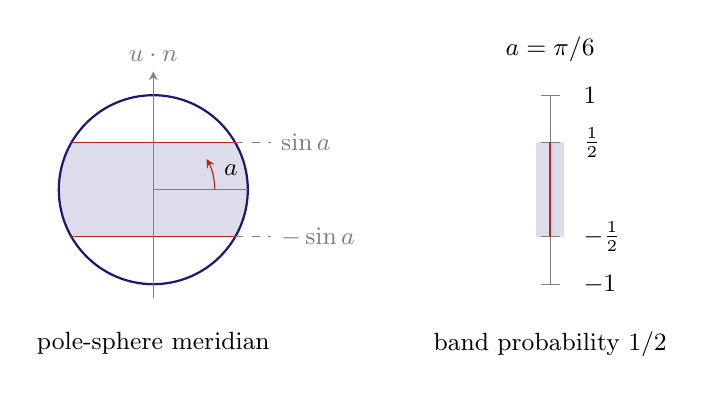
\begin{tikzpicture}[x=1.2cm,y=1.2cm,font=\small,>=stealth]
\begin{scope}
\clip (0,0) circle (1);
\fill[MidnightBlue!15] (-1,-.5) rectangle (1,.5);
\end{scope}
\draw[MidnightBlue,thick] (0,0) circle (1);
\draw[BrickRed] (-.8660254,.5)--(.8660254,.5);
\draw[BrickRed] (-.8660254,-.5)--(.8660254,-.5);
\draw[gray,->] (0,-1.15)--(0,1.25) node[above] {$u\cdot n$};
\draw[gray] (0,0)--(1,0);
\draw[BrickRed,->] (.65,0) arc[start angle=0,end angle=30,radius=.65];
\node at (.82,.21) {$a$};
\draw[gray,dashed] (.8660254,.5)--(1.25,.5) node[right] {$\sin a$};
\draw[gray,dashed] (.8660254,-.5)--(1.25,-.5) node[right] {$-\sin a$};
\node[below] at (0,-1.4) {pole-sphere meridian};
\begin{scope}[shift={(4.2,0)}]
\fill[MidnightBlue!15] (-.15,-.5) rectangle (.15,.5);
\draw[gray] (0,-1)--(0,1);
\foreach \z/\lab in {-1/-1,-.5/{-\frac12},.5/{\frac12},1/1} {
\draw[gray] (-.1,\z)--(.1,\z);
\node[right] at (.25,\z) {$\lab$};}
\draw[BrickRed,thick] (0,-.5)--(0,.5);
\node[above] at (0,1.25) {$a=\pi/6$};
\node[below] at (0,-1.4) {band probability $1/2$};
\end{scope}
\end{tikzpicture}
